\def\probtitle{산책과 쿼리}
\def\probno{I}

\begin{problem}{\probno{}. \probtitle{}}

성서는 숭실대학교 근처 자취 후보 장소를 $N$개 선정해 $1$부터 $N$까지 번호를 붙였다. 각 장소에는 자취방이 정확히 하나씩 있다. 자취방을 구할 때 고려할 사항은 여러 가지가 있지만, 성서는 그중에서도 산책의 자유도를 가장 중요하게 생각한다.

\textbf{산책로} $(a, b)$는 서로 다른 두 장소 $a$와 $b$를 잇는 길로, $a$에서 $b$로 걷는 데 $1$의 시간이 걸리고, $b$에서 $a$로 걷는 데에도 $1$의 시간이 걸린다. 일단 걷기 시작하면 중간에 방향을 꺾거나 멈추지 않고 정확히 $1$의 시간 동안 걸어서 반대편에 도착해야 한다.

\textbf{산책}은 어떤 장소 $u$에서 출발해 산책로를 따라 걸어 다니다가 마지막에 다시 $u$로 되돌아오는 행동이다. 산책 도중에 어떤 장소나 산책로를 여러 번 방문해도 되지만, 산책 도중에 잠시라도 걸음을 멈추면 안 된다.

성서는 장소들 사이를 둘러보며 분위기가 좋은 산책로들을 자신만의 산책로 리스트에 추가할 계획이다. \textbf{만족스러운 산책}이란, 산책로 리스트에 적힌 산책로만을 사용하는 산책이다.

성서는 충분히 긴 시간 동안 산책을 하다가 원하는 시간에 맞춰 되돌아오고 싶다. 어떤 자취방 $u$가 \textbf{산책의 자유도가 높다}는 것은, $10^6$ 이상의 어떤 정수 $t$를 고르더라도, 장소 $u$에서 출발하면서 정확히 $t$의 시간이 걸리는 만족스러운 산책이 존재함을 의미한다.

처음에는 산책로 리스트가 비어 있지만, 성서는 분위기가 좋은 산책로를 발견할 때마다 그 산책로를 리스트에 추가할 것이다. 리스트가 변경될 때마다 산책의 자유도가 높은 자취방이 몇 개나 있는지 알아보자.

구체적으로, 다음과 같은 쿼리를 $Q$번 처리해야 한다.
\begin{itemize}
    \item \texttt{a b}: 산책로 $(a, b)$를 산책로 리스트에 추가한다. 이후 산책의 자유도가 높은 자취방의 개수를 출력한다.
\end{itemize}

\begin{center}
    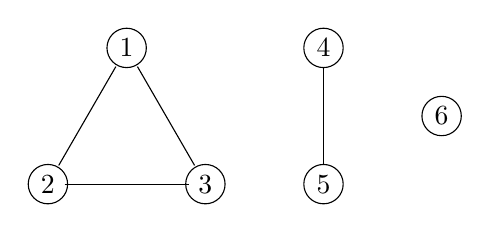
\begin{tikzpicture}
        \node (1) at (0, 1.73) {1};
        \node (2) at (-1, 0) {2};
        \node (3) at (1, 0) {3};
        \node (4) at (2.5, 1.73) {4};
        \node (5) at (2.5, 0) {5};
        \node (6) at (4, 0.865) {6};
        \draw (1) -- (2);
        \draw (1) -- (3);
        \draw (2) -- (3);
        \draw (4) -- (5);
        \path[draw=black] (1) circle[radius=0.25];
        \path[draw=black] (2) circle[radius=0.25];
        \path[draw=black] (3) circle[radius=0.25];
        \path[draw=black] (4) circle[radius=0.25];
        \path[draw=black] (5) circle[radius=0.25];
        \path[draw=black] (6) circle[radius=0.25];
    \end{tikzpicture}
\end{center}

% \textbf{\textcolor{red}{@TODO 예시 그림 추가}}

예를 들어 자취방이 $6$개이고 산책로 리스트가 $\{(1,2), (2,3), (1,3), (4,5)\}$라면 위 그림처럼 표현할 수 있다.

자취방 $6$에서는 $10^6$의 시간이 걸리는 만족스러운 산책을 할 수 없으므로 산책의 자유도가 높지 않다.

자취방 $4$와 $5$에서는 $10^6$이나 $10^6+2$ 등의 시간이 걸리는 만족스러운 산책은 할 수 있지만, $10^6+1$이나 $10^6+3$ 등의 시간이 걸리는 만족스러운 산책은 할 수 없으므로 산책의 자유도가 높지 않다.

반면에 자취방 $1,2,3$은 $10^6$이나 $10^6+1, 10^6+2, 10^6+3, \cdots$의 시간이 걸리는 만족스러운 산책이 모두 가능하므로 산책의 자유도가 높다.

따라서 위 그림에서 산책의 자유도가 높은 자취방의 개수는 $3$이다.

\InputFile

첫째 줄에 장소의 개수 $N$과 쿼리의 개수 $Q$가 공백으로 구분되어 주어진다.

둘째 줄부터 $Q$개의 줄에 걸쳐, $i$번째 줄에 $i$번째 쿼리에서 추가되는 산책로가 연결하는 두 장소 $a_i, b_i$가 공백으로 구분되어 주어진다.

\OutputFile

쿼리가 주어질 때마다 한 줄에 하나씩 정답을 출력한다.

\Constraints

\begin{itemize}[noitemsep]
    \item $2 \leq N \leq 3 \times 10^5$
    \item $1 \leq Q \leq 6 \times 10^5$
    \item $1 \leq a_i < b_i \leq N$ $(1 \le i \le Q)$
    \item 동일한 쿼리가 여러 번 주어지지 않는다.
    \item 주어지는 수는 모두 정수이다.
\end{itemize}

\Example

\begin{example}
    \exmpfile{./example/01.in.txt}{./example/01.out.txt}%
    \exmpfile{./example/02.in.txt}{./example/02.out.txt}%
\end{example}

% \newpage

\Notes
입출력 양이 많으므로 문제지 2--4페이지의 언어 가이드에 있는 빠른 입출력을 사용하는 것을 권장한다.

\end{problem}